%!TEX root = ../problems.tex
\begin{task}
	Найти спектр сигнала, изображенного на рисунке. Построить график $|S(w)|$.
\end{task}
\begin{figure}[ht]
  \centering
  \begin{subfigure}[b]{0.5\linewidth}
    \centering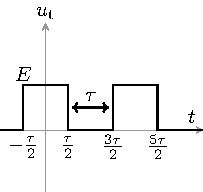
\includegraphics[scale=2]{ris/task9_input}
	\label{fig:9}
    \caption{\label{fig:fig9}}
  \end{subfigure}%
  \begin{subfigure}[b]{0.5\linewidth}
    \centering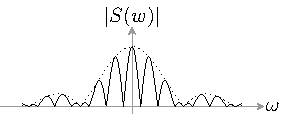
\includegraphics[scale=2]{ris/task9_out}
    \caption{\label{fig:fig9.1}}
    \label{fig:9.1}
  \end{subfigure}%
  \caption{Сигнал \subref{fig:fig9} и найденный его спектр \subref{fig:fig9.1}}
\end{figure}

\begin{proof}[\rm{\textbf{Решение}}]
В силу линейности преобразования Фурье, представив сигнал как сумму двух прямоугольных импульсов $u(t) = u_1(t)+u_2(t)$,получим:
\begin{equation}
	S(w) = S_1(w) +S_2(w),
\end{equation}
где $S_1 \LT u_1(t)$ и $S_2 \LT u_2(t)$.

Кроме того, можно вспомнить, что спектр единичного прямоугольного импульса, симметричного относительно момента времени $t=0$,  $S(w) = A\tau\frac{\sin{\frac{w\tau}{2}}}{\frac{w\tau}{2}} = A\tau ~ \mathrm{sinc}(\frac{w\tau}{2}) $. Очевидно, $S_1=S$, а второй импульс просто сдвинут на время $2\tau$, и из свойств преобразования Фурье это просто дает экспоненту в образе: 
\begin{equation}
	S(w) = S_1(w) +S_2(w) = S(w)\qty(1+e^{-2\cdot iw\tau}),
\end{equation}
Тогда, свернув сумму экспонент по формуле Эйлера, получим:
\begin{equation}
	 {S(w)} = A\tau~\mathrm{sinc}\qty(\frac{w\tau}{2}) \cdot e^{-iw\tau}\frac22\qty(e^{-iw\tau}+e^{iw\tau}) =
	2A\tau~\mathrm{sinc}\qty(\frac{w\tau}{2}) \cdot e^{-iw\tau} \cos{w\tau}
\end{equation}
И окончательный ответ
\begin{equation}
	|S(w)| = 2A\tau~ \abs{\mathrm{sinc}~\qty(\frac{w\tau}{2})  \cos{w\tau}}
\end{equation}

\end{proof}